\chapter{Methodology Results and Discussion}

% Materials and Methods is the chronological listing of steps and procedure/s used by the proponent/s.
% Methods used for gathering of data, laboratory and field experiment, theoretical and/or conceptual frameworks, as well as techniques employed in the analyses of data must be specifically listed.

\section{Software Design}

The software design of the proposed system is represented by the following Hierarchical Input-Process-Output (HIPO) diagrams.

\vspace{1cm}

\begin{figure}[h!]
    \begin{center}
        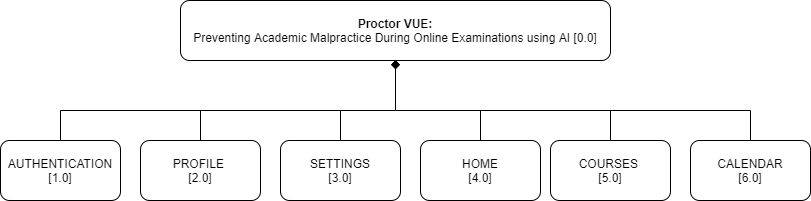
\includegraphics[scale=0.8]{main-hipo}
        \caption{Proctor Vue HIPO}
    \end{center}
\end{figure}

\vspace{1cm}

\begin{figure}[h!]
    \begin{center}
        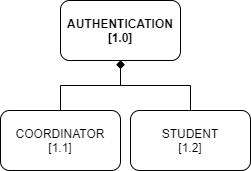
\includegraphics[scale=0.7]{auth-hipo.png}
        \caption{Authentication}
    \end{center}
\end{figure}

\vspace{1cm}

\begin{figure}[h!]
    \begin{center}
        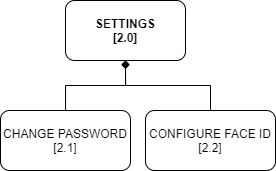
\includegraphics[scale=0.7]{settings-hipo.png}
        \caption{Settings}
    \end{center}
\end{figure}

\vspace{1cm}

\begin{figure}[h!]
    \begin{center}
        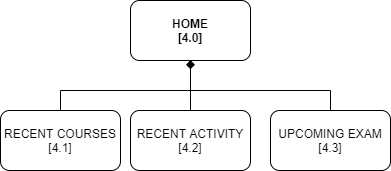
\includegraphics[scale=0.7]{home-hipo.png}
        \caption{Home Page}
    \end{center}
\end{figure}

\vspace{1cm}

\begin{figure}[h!]
    \begin{center}
        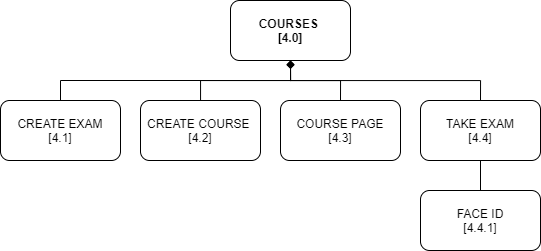
\includegraphics[scale=0.7]{courses-hipo.png}
        \caption{Courses}
    \end{center}
\end{figure}

\section{System Architecture}
The following diagram represents the system architecture of the proposed system.

\begin{figure}[h!]
    \begin{center}
        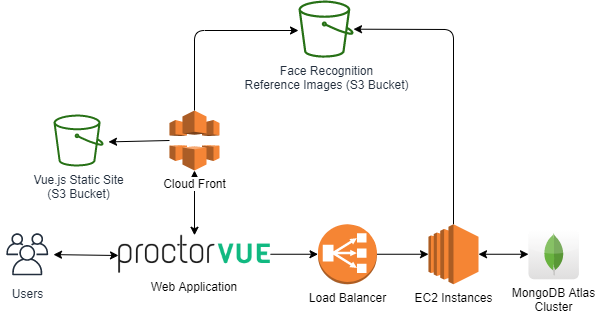
\includegraphics[scale=0.75]{sys-arch.png}
        \caption{System Architecture of Proctor Vue}
    \end{center}
\end{figure}

\section{Cost Benefit Analysis}

This following estimates the cost of software required by the proposed system.

% \noindent
% \textbf{Software Development Cost}

% \begin{table}[h!]
%     \begin{center}
%         \begin{tabular}{|l|c|r|}
%             \hline
%             \textbf{Personnel}                   & \textbf{No. of Personnel} & \textbf{Salary} \\
%             \hline
%             Programmer                           & 1                         & \PHP20,000.00   \\
%             \hline
%             System Analyst                       & 1                         & \PHP35,000.00   \\
%             \hline
%             \multicolumn{2}{|l|}{\textbf{Total}} & \textbf{\PHP55,000.00}                      \\
%             \hline
%         \end{tabular}
%     \end{center}
%     \caption{Software Development Cost}
% \end{table}

% \noindent
% \textbf{System Cost}

\pagebreak

\begin{table}[h!]
    \begin{center}
        \begin{tabular}{|l|c|r|}
            \hline
            \textbf{Item}                        & \textbf{Specification}       & \textbf{Cost} \\
            \hline
            Datebase Instance                    & MongoDB Atlas                & \PHP2,805.81  \\
            \hline
            Storage for User-Uploaded Images     & Amazon S3/CloudFront         & \PHP32.15     \\
            \hline
            Web Application Hosting              & Amazon S3/CloudFront         & \PHP454.82    \\
            \hline
            Load Balancer                        & Amazon Elastic Load Balancer & \PHP896.30    \\
            \hline
            Application Backend and API          & Amazon EC2                   & \PHP4,246.70  \\
            \hline
            \multicolumn{2}{|l|}{\textbf{Total}} & \textbf{\PHP8,435.78}                        \\
            \hline
        \end{tabular}
    \end{center}
    \caption{System Cost}
\end{table}

Source: www.mongodb.com, calculator.aws

\section{Requirement Analysis}
The following Data-Flow Diagram (DFD) illustrates the requirements needed to build and develop the proposed system.

\begin{figure}[h!]
    \begin{center}
        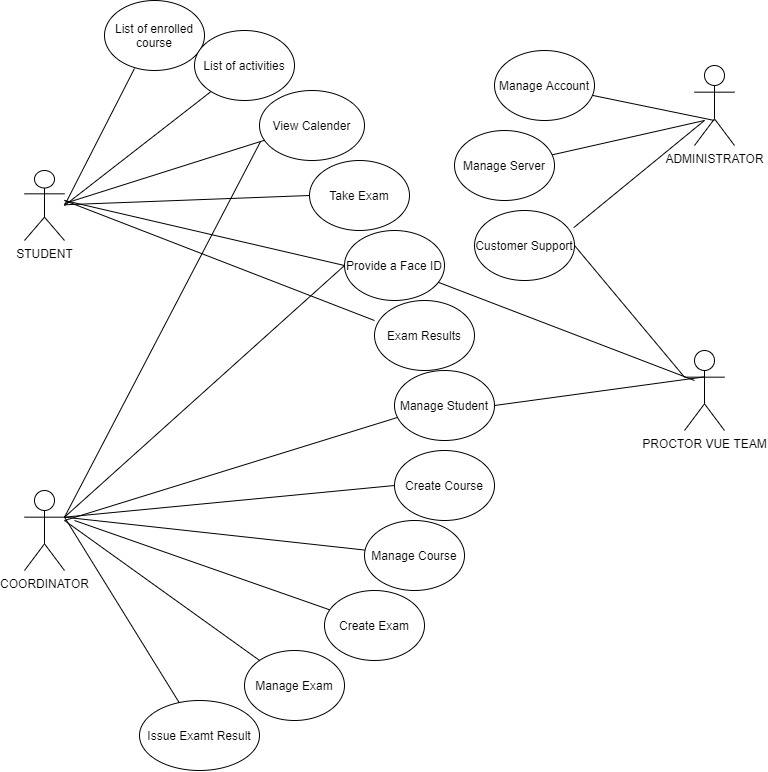
\includegraphics[scale=0.3]{dfd.jpg}
        \caption{Data Flow Diagram of the Proposed System}
    \end{center}
\end{figure}

\section{Block Diagrams}

\begin{figure}[h!]
    \begin{center}
        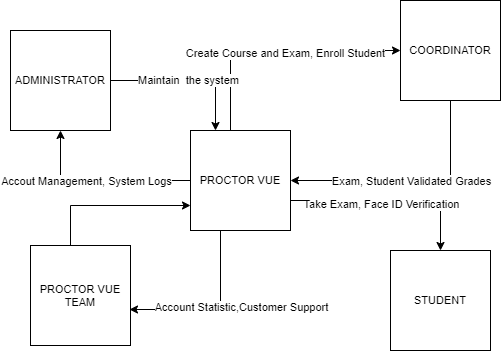
\includegraphics[scale=0.8]{block.png}
        \caption{Block Diagram of the Proposed System}
    \end{center}
\end{figure}

As illustrated by the block diagram, there are four key actors involved in the system's overall process.
Administrators oversee the whole system, handling the different types of accounts as well as assigning them their roles.
Coordinators handle courses by creating new courses, managing active courses, and creating \& scheduling exams.
Students will be enrolled by each course's coordinator.
Once enrolled, they can take available exams.

\section{Development and Testing}

The proposed system adheres to standard conventions in developing a full-stack web application.
The backend API follows conventions for RESTful APIs in order to have a clear and consistent semantic meaning when interfacing with the application.

To aid in development, various unit tests were written alongside new incremental additions to the application and its API.
The entire application's tests were written using Jest, a popular JavaScript testing framework.
The API endpoints were tested using Jest and SuperTest, which allows for testing HTTP requests.
These tests ensure that the system runs as expected and is integrated continuosly with existing components.

\section{Input and Output Reports and Analysis}

\begin{figure}[h!]
    \begin{center}
        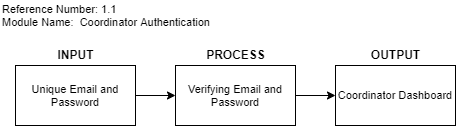
\includegraphics[scale=0.8]{coordinator-auth-ipo.png}
        \caption{Coordinator Authentication}
    \end{center}
\end{figure}

\begin{figure}[h!]
    \begin{center}
        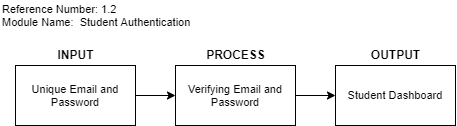
\includegraphics[scale=0.8]{student-auth-ipo.png}
        \caption{Student Authentication}
    \end{center}
\end{figure}

\pagebreak

\begin{figure}[h!]
    \begin{center}
        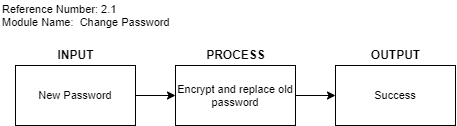
\includegraphics[scale=0.8]{change-password-ipo.png}
        \caption{Change Password IPO}
    \end{center}
\end{figure}

\begin{figure}[h!]
    \begin{center}
        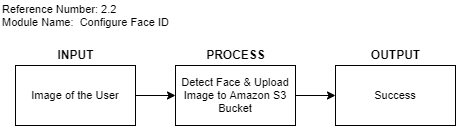
\includegraphics[scale=0.8]{configure-face-id-ipo.png}
        \caption{Configure Face ID IPO}
    \end{center}
\end{figure}

\begin{figure}[h!]
    \begin{center}
        
\includegraphics[scale=0.8]{recent-courses-ipo.png}
        \caption{Recent Courses IPO}
    \end{center}
\end{figure}

\pagebreak

\begin{figure}[h!]
    \begin{center}
        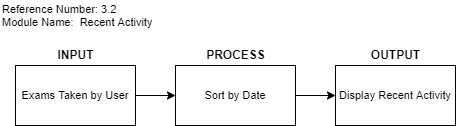
\includegraphics[scale=0.8]{recent-activity-ipo.png}
        \caption{Recent Activity IPO}
    \end{center}
\end{figure}

\begin{figure}[h!]
    \begin{center}
        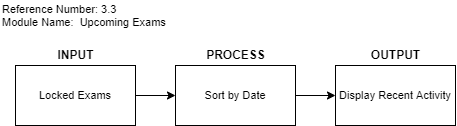
\includegraphics[scale=0.8]{upcoming-exams-ipo.png}
        \caption{Upcoming Exams IPO}
    \end{center}
\end{figure}

\begin{figure}[h!]
    \begin{center}
        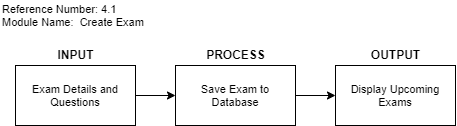
\includegraphics[scale=0.8]{create-exam-ipo.png}
        \caption{Create Exam IPO}
    \end{center}
\end{figure}

\pagebreak

\begin{figure}[h!]
    \begin{center}
        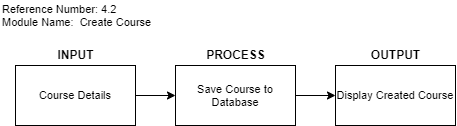
\includegraphics[scale=0.8]{create-course-ipo.png}
        \caption{Create Course IPO}
    \end{center}
\end{figure}

\begin{figure}[h!]
    \begin{center}
        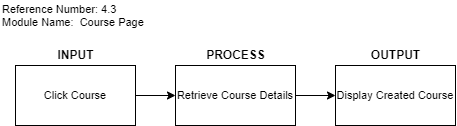
\includegraphics[scale=0.8]{course-page-ipo.png}
        \caption{Course Page IPO}
    \end{center}
\end{figure}

\begin{figure}[h!]
    \begin{center}
        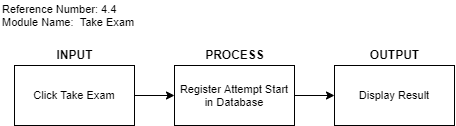
\includegraphics[scale=0.8]{take-exam-ipo.png}
        \caption{Take Exam IPO}
    \end{center}
\end{figure}

\pagebreak

\begin{figure}[h!]
    \begin{center}
        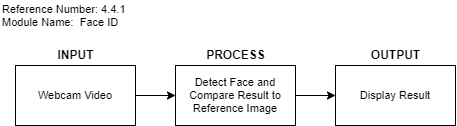
\includegraphics[scale=0.8]{face-id-ipo.png}
        \caption{Face ID IPO}
    \end{center}
\end{figure}

\section{Description of the Prototype}

Proctor Vue will implement facial detection/recognition during online exams for different courses.
These exams will be created by the assigned coordinator in each course through Proctor Vue.
Before users can take the exams, they must provide an image of themselves in order for the camera to ensure they are the ones present for their examination.
During an exam, the student's face must be seen and recognized as the provided image every minute or else they will incur a warning.
Maxing out the set number of warnings for the exam will automatically fail the student for that attempt.

\section{Implementation Plan}

The developed system will be sent to AMA Computer College Parañaque right away after the revision to present it once more to the end users.
If the company wants to adopt the proposed system, the proponents will hand over the system together with its documentation which will serve as a guide to the Administrator who will be assigned for the system’s update and maintenance.
There will be a letter of agreement that the system will be handed over to the company freely and the researchers are no longer responsible for the updates and maintenance.
If the system will be implemented, the researchers will conduct several strategies as presented below

\vspace{1cm}

\begin{table}[h!]
    \begin{center}
        \begin{tabular}{|m{10em}|m{8em}|m{10em}|m{4em}|}
            \hline
            \textbf{Strategy}        & \textbf{Activities}              & \textbf{Persons Involved}         & \textbf{Duration} \\
            \hline
            Approval from Admin      & Send letter to Admin             & Researchers \& Admin              & 1 Day             \\
            \hline
            Information distribution & Provide techinical documentation & Researchers \& Admin              & 1 Day             \\
            \hline
            3 Days training          & Training for users               & Researchers \& Admin \& Employees & 3 Days            \\
            \hline
        \end{tabular}
    \end{center}
    \caption{Implementation Plan}
\end{table}

\section{Algorithm Use}

Proctor Vue utilizes an open source high-level face detection library, \lstinline{face-api.js}.
Under the hood, the library implements facial detection and recognition using different machine learning algorithms to cater to different use cases.

For the proposed system, the Tiny Face Detector neural network is used to perform fast facial detection in the browser.

The Tiny Face Detector model is more performant and less resource intensive compared to another well-known neural network for face detection, Single Shot Multibox Detector.
It makes intuitive use of different factors such as scale, resolution, and context for object detection.
In a research made by the original developers of the neural network, they found that the model can detect approximately 80\% of 1000 faces in a large image \cite{Hu_2017_CVPR}.

The facial recognition model, under the hood, is implemented using a residual network.
In practice, it will compute a descriptor for a person's face, describing their face's unique characteristics.
The model has an accuracy of 99.38\% in a facial recognition benchmark test.
